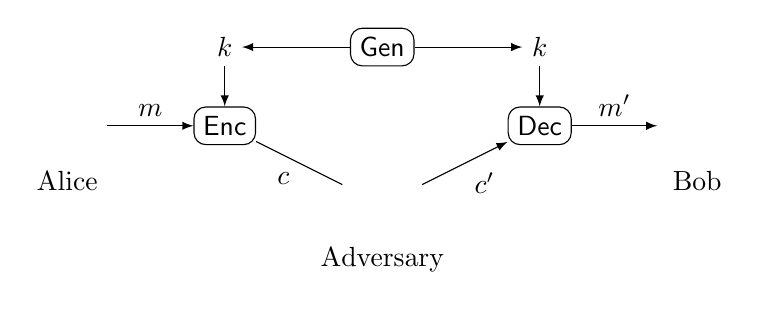
\begin{tikzpicture}
\node (sender) [minimum size=1cm] {}; \Alice{0}{0}{0.4};
\node (bart) [below of = sender, node distance = 0.7cm] {Alice};
\node (enc) [draw, right of = sender, rounded corners=1ex,node distance = 2cm] {$\mathsf{Enc}$};
\node (k1) [above of = enc, node distance = 1cm] {$k$};
\node (c) [right of = enc, node distance = 2cm] {};
\node (gen) [draw, above of = c, rounded corners=1ex,node distance = 1cm] {$\mathsf{Gen}$};
\node (adv) [below of = c, node distance = 1cm, minimum size=1cm] {}; \Evil{4cm}{-1cm}{0.4};
\node (burns) [below of = adv, node distance = 0.7cm] {Adversary};
\node (dec) [draw, right of = c, rounded corners=1ex,node distance = 2cm] {$\mathsf{Dec}$};
\node (k2) [above of = dec, node distance = 1cm] {$k$};
\node (receiver) [right of = dec, node distance = 2cm, minimum size=1cm] {}; \Bob{8cm}{0}{0.4};
\node (lisa) [below of = receiver, node distance = 0.7cm] {Bob};
\draw[-latex] (sender) -- (enc) node [midway, above] {$m$};
\draw (enc) to node [auto,swap] {$c$} (adv); \draw[-latex] (adv) to node [auto,swap] {$c'$} (dec);
\draw[-latex] (dec) -- (receiver) node [midway, above] {$m'$};
\draw[-latex] (k1) -- (enc);
\draw[-latex] (gen) -- (k1);
\draw[-latex] (gen) -- (k2);								
\draw[-latex] (k2) -- (dec);		
\end{tikzpicture}